\documentclass[conference]{IEEEtran}
\IEEEoverridecommandlockouts
% The preceding line is only needed to identify funding in the first footnote. If that is unneeded, please comment it out.
%\usepackage{cite}
\usepackage{amsmath,amssymb,amsfonts}
\usepackage{algorithmic}
\usepackage{graphicx}
\usepackage{textcomp}
\usepackage[table,xcdraw]{xcolor}
\usepackage{paralist} % compactitem etc
\usepackage{booktabs} % For formal tables
\usepackage{numprint}
\usepackage{xspace}
%\usepackage{cite}
\usepackage{amsmath,amssymb,amsfonts}
\usepackage{color}
\usepackage{textcomp}
\usepackage[normalem]{ulem}
\usepackage{soul}
\usepackage{multirow}
\usepackage{multicol}
\usepackage{footmisc}
\usepackage{dblfloatfix}
\usepackage{listings}
\usepackage[utf8]{inputenc}
\usepackage[english]{babel}
\usepackage[noadjust]{cite}
\usepackage{listings}
\usepackage{minted}
\usepackage{amsthm}
\usepackage{amssymb}
\usepackage{pdfrender}

% If you use beamer only pass "xcolor=table" option, i.e. \documentclass[xcolor=table]{beamer}
\usepackage[normalem]{ulem}
\useunder{\uline}{\ul}{}

\usepackage[table,xcdraw]{xcolor}
%\usepackage[noline,noend]{algorithm2e}
\usepackage[noline]{algorithm2e}
\usepackage{url}
\def\UrlFont{\rmfamily}

\usepackage[colorinlistoftodos]{todonotes}
\newcommand{\ignore}[1]{ } % ignore blocks of text
\newcommand{\maketiny}[1]{{\tiny G: #1}} % ignore blocks of text
\newcommand{\ganesh}[1]{\todo[inline,size=\small, color=purple!40]{G: #1}}



\newcommand{\goat}{\textsc{GoAT}\xspace}

\newcommand{\etc}{etc.\@\xspace}
\newcommand{\ie}{i.e.\@\xspace}
\newcommand{\eg}{e.g.\@\xspace}

%% colors
\newcommand{\tbl}[1]{\textcolor{blue}{#1}}
\newcommand{\tb}[1]{\textcolor{black}{#1}}
\newcommand{\tr}[1]{\textcolor{red}{#1}}
\newcommand{\tg}[1]{\textcolor{green}{#1}}

\newcommand\ggcmt[1]{\todo[inline, size=\small, color=green!40]{GG: #1}}
\newcommand\ggcmtside[1]{\todo[size=\scriptsize, color=green!40]{GG: #1}}

\newcommand\stcmt[1]{\todo[inline, size=\small, color=orange!60]{#1}}
\newcommand\stcmtside[1]{\todo[size=\scriptsize, color=orange!40]{#1}}

%--\newcommand{\circleRtool}{circleRtool\circledR\xspace}

%%% Local Variables:
%%% mode: latex
%%% eval: (flyspell-mode 1)
%%% TeX-master: "root.tex"
%%% End:


\renewcommand{\algorithmcfname}{Procedure}




\newtheorem{definition}{Definition}[section]

\makeatletter
\def\BState{\State\hskip-\ALG@thistlm}
\makeatother

\definecolor{codegreen}{rgb}{0,0.3,0}
\definecolor{codegray}{rgb}{0.5,0.5,0.5}
\definecolor{codepurple}{rgb}{0.58,0,0.82}
\definecolor{backcolour}{rgb}{0.98,0.98,0.98}

\lstdefinestyle{mystyle}{
    backgroundcolor=\color{backcolour},
    commentstyle=\color{codegreen},
    keywordstyle=\color{magenta},
    numberstyle=\tiny\color{codegray},
    stringstyle=\color{codepurple},
    basicstyle=\ttfamily\scriptsize,,
    breakatwhitespace=false,
    breaklines=true,
    captionpos=b,
    keepspaces=true,
    numbers=left,
    numbersep=4pt,
    showspaces=false,
    showstringspaces=false,
    showtabs=false,
    tabsize=2,
    morekeywords={pragma, omp}
}

\lstset{style=mystyle}
\lstset{escapeinside={<@}{@>}}



\def\BibTeX{{\rm B\kern-.05em{\sc i\kern-.025em b}\kern-.08em
    T\kern-.1667em\lower.7ex\hbox{E}\kern-.125emX}}
\begin{document}


\title{\goat: Automated Dynamic Concurrency Analysis and Testing for Go}


\author{\IEEEauthorblockN{Saeed Taheri}
\IEEEauthorblockA{\textit{School of Computing} \\
\textit{University of Utah}\\
Salt Lake City, U.S.A. \\
staheri@cs.utah.edu}
\and
\IEEEauthorblockN{Ganesh Gopalakrishnan}
\IEEEauthorblockA{\textit{School of Computing} \\
\textit{University of Utah}\\
Salt Lake City, U.S.A. \\
ganesh@cs.utah.edu}
}

\maketitle

\begin{abstract}


\end{abstract}

\begin{IEEEkeywords}
golang, concurrency, testing coverage analysis
\end{IEEEkeywords}

\section{GIntroduction}
\label{sec:Gintro}

Increasing levels of parallelism and concurrency in HPC and Cloud---both
at the user program level and in the infrastructure---leads to concurrency
bugs which are high up among the root-causes for lost productivity.
%
This trend will only worsen with the upcoming HPC/Cloud
integration~\cite{dan-herbein-dong}.
%
Unless simple and effective concurrency analysis and
debugging methods are employed at all levels of
concurrency, one will face the complexity of maintaining
the debugging ecosystem in addition to the codebase itself.


Motivated by these considerations,
in this study we take the feature-rich language, namely Go,
and offer a combined static and dynamic approach for debugging
Go programs.
%
Not only is Go gaining in acceptance in the Cloud community,
it also involves shared memory, message passing, nondeterminism
and dynamic process creation in a manner that makes debugging hard.
%
Our work is especially relevant
because Go is a language that has leapfrogged tooling support: not only
are there no widely usable tools for debugging Go, even well-curated
bug benchmark suites are only just now beginning to appear \cite{tu-concurrentBugs-asplos19,yuan-gobench-cgo21}.
%
Combinations of Go's features are found in many other languages,
making our study carry a broader degree of relevance
to the HPC/Cloud ecosystem, in addition to providing an effective
tool for Go itself.


Given the extent of lack of verification support, one of
our priorities was to reuse as much of the existing Go infrastructure
as we could.
%
The static analysis component relies on source rewriting, inserting
{\em potential} schedule yield points
at all
``interesting'' (concurrency-relevant) spots inside a given Go program.
%
The dynamic component consists of yielding control back
to the Go runtime with a user-settable probability value. \stcmtside{also tracing}


Our preliminary results in terms of this combined static/dynamic
approach yielded encouraging results.
%
However, bug-hunting on curated bug data sets do not give any
indications on how well this approach can {\em generalize}.
%
Generalization in terms of debugging tools is often achieved
by carefully defining {\em coverage metrics} and showing how
well these metrics are met.
%
Again, we walked into a field with very few such coverage metrics.

\stcmt{ about below statement: the coverage metrics that we designed is brand new. It is inspired by other concurrrency metrics but new ideas are generated. Also coverage metrics for select statement are purely ours. There is no mention of select statements as the root cause of rare bugs anywhere in the literature. Based on our vision from studying bug kernels using dynamic tracing, we came up with new coverage metrics.}
Our design of coverage metrics proceeded
by observing the preponderance
of reported Go bugs in recent studies.
%
Informed by these studies,
we define {\em coverage metrics} by reusing
(and extending)
well known concurrency metrics in related work.
%
We take advantage of our own tracing framework to
tabulate and report on the achieved coverage metrics.
%
All this is offered via a new tool called \goat (Go Analysis and Testing Tool)
that we now describe, after introducing relevant features of Go
itself.

\noindent{\bf Features of Go:\/}
Go \cite{go} is a statically typed language initially developed by Google and at present widely used by many.
%
It employs channel-based Hoare's Communicating Sequential Processes (CSP) \cite{hoare-csp78} semantics in its core and provides a productivity-enhancing environment for concurrent programming.
%
The concurrent model in Go centers around
1) \textit{goroutines} as light-weight user-level threads (processing units),
2) \textit{channels} for explicit messaging to synchronize and share memory through communication, and
3) a \textit{scheduler} that orchestrates goroutine interactions while shielding
the user from
many low-level
aspects of the runtime.
%
This design
facilitates the
construction
of data flow models that efficiently utilize multiple CPU cores.
%
Because of the simple yet powerful concurrency model, many real production software systems take advantage of Go,
including
container software systems such as Docker \cite{merkel2014docker}, Kubernetes \cite{kubernetes},  key-value databases \cite{etcd}, and web server libraries \cite{grpc}.
%


In traditional shared-memory concurrent languages such as Java/C/C++, threads interact with each other via shared memory.
%
Processes in CSP-based languages such as Erlang communicate through mailbox (asynchronous) message passing.
%
Go brings all these features together into one language and encourages developers to \textit{share memory through communication} for safe and straightforward concurrency and parallelism.
%
The visibility guarantee of memory writes is specified in the memory model\cite{go-memModel} under synchronization constraints (\textit{happens-before} partial order \cite{lamport-hb-1978}).
%
The language is equipped with a rich vocabulary of \textit{serialization} features to facilitate the memory model constraints; they include synchronous and asynchronous communication (either unbuffered or buffered channels), memory protection, and barriers for efficient synchronization.
%
This rich mixture of features has, unfortunately, greatly exacerbated the complexity of Go debugging.
%
In fact, the popularity of Go has outpaced its debugging support~\cite{go-survey,tu-concurrentBugs-asplos19,dilley-empirical-saner19}.
%
There are some encouraging developments in support of debugging, such as a data race checker \cite{go-race-blog} that has now become a standard feature of Go, and has helped catch many a bug.
%
However, the support for ``traditional concurrency debugging'' such as detecting atomicity violations and Go-specific bug-hunting support for Go idioms (e.g., misuse of channels and locks) remain insufficiently addressed.
%

\noindent{\bf Contributions:\/} In
this work, we present the initial steps that we took towards addressing this lack.
%
Since a bug might
occur
at various levels of abstraction, dynamic tracing provides a practical and uniform way to track multiple facets of the program during execution (as we have shown in our prior work~\cite{difftrace}).
%
Also, unlike assertion-based tools \cite{lange-staticType-icse18,wolf-gobra-cav21}, a dynamic tool is more automated, not requiring user expertise.
%
We developed a facility that automatically gathers \textit{execution concurrency traces} (\ie sequences of events) during the execution of Go applications with minimal instrumentation.
%
By enhancing the Go built-in tracing mechanism with \textit{concurrency usage} events, we enrich original \textit{execution traces} so that they accurately reflect the dynamic concurrency behavior of applications.
%
Upon Go programs' termination when tracing is enabled, traces are flushed and structurally stored in relational tables of an SQL database, enabling multi-aspect program analysis in offline.
%

With the help of this novel \textit{automated dynamic tracing} mechanism,
we have implemented a testing framework that
\textit{accelerates} bug exposure by manipulating the native scheduler around \textit{critical points} in the code---combination of constructs that heighten the propensity for bug-introduction.
%



To summarize, here are our contributions:
\stcmtside{need to update}
\begin{itemize}
    \item We take the tracing mechanism embedded in the standard Go that captures \textit{execution trace} (ET) and enhance it with a set of concurrency primitive usage events to obtain \textit{execution concurrency trace} (ECT). While the primary usage of ET is performance analysis, ECT provides an accurate and comprehensive model of concurrent execution, enabling automated analysis of logical behavior and concurrent bug detection.
    \item We introduce a framework that automatically instruments the target program, collects ECT, and structurally stores them in a database. Through querying the database, several visualizations and reports are accessible.
    \item We propose an approach to identify the points (\ie source line number) in the target program in which a random noise might drastically change the program's dynamic behavior. We analyze ECTs to identify such points and measure schedule space coverage per execution.
    \item Coverage metric
\end{itemize}
\stcmtside{need to update}
The rest of this paper is as follows: Section \ref{sec:correctness} discusses correctness problems and approaches in Go. Section \ref{sec:ect} describes the enhancement we made to the tracer package. Section \ref{sec:disc} discusses the advantages of dynamic tracing for concurrent debugging and draws the ongoing and future direction of the current work. At last, section \ref{sec:summary} summarizes and concludes.


\section{Background}
\label{sec:bg}

\begin{listing*}[]
\begin{minipage}{.35\textwidth}
\begin{minted}
[
fontsize=\footnotesize,
linenos=true,
escapeinside=||,
breaklines
]
{go}
package main
import "sync"

type Container struct{ |\label{bugListing:containerType_start}|
  sync.Mutex
  stop  chan struct{}
} |\label{bugListing:containerType_end}|

func main() {
  container := &Container{ |\label{bugListing:container_create_start}|
       stop:make(chan struct{})} |\label{bugListing:container_create_end}|
  go Monitor(container) |\label{bugListing:main_go_monitor}|
  go StatusChange(container) |\label{bugListing:main_go_statChange}|
}
\end{minted}
\end{minipage}
\begin{minipage}{.35\textwidth}
\begin{minted}
[
fontsize=\scriptsize,
linenos=true,
escapeinside=||,
breaklines
]
{go}
|\setcounter{FancyVerbLine}{15}|func Monitor(cnt *Container){
  for{
    select{|\label{bugListing:Monitor_select}|
    case <- cnt.stop:  |\label{bugListing:Monitor_case_recv}|
      return |\label{bugListing:Monitor_case_recv_ret}|
    default: |\label{bugListing:Monitor_case_def}|
      cnt.Lock()  |\label{bugListing:Monitor_case_def_lock}|
      cnt.Unlock() |\label{bugListing:Monitor_case_def_unlock}|
}}}
func StatusChange(cnt *Container){
  cnt.Lock() |\label{bugListing:statChange_lock}|
  defer cnt.Unlock() |\label{bugListing:statChange_defer_unlock}|
  cnt.stop <- struct{}{} |\label{bugListing:statChange_send}|
}
\end{minted}
\end{minipage}
\begin{minipage}{.25\textwidth}
  \centering
  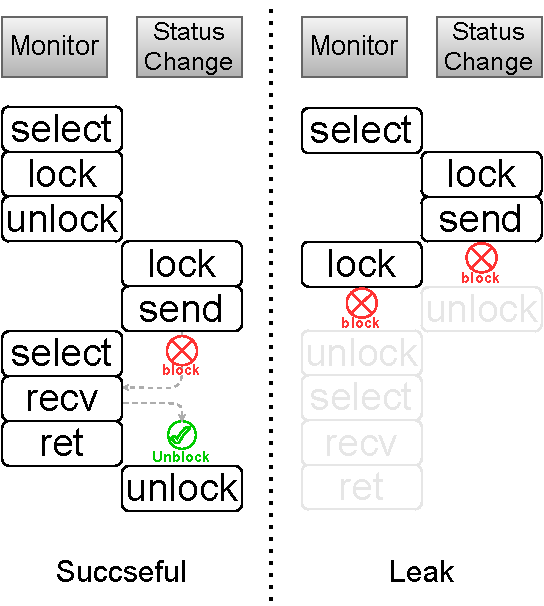
\includegraphics[width=.99\linewidth]{figs/execViz_moby.pdf}
\end{minipage}
\caption{Simplified version of bug \texttt{moby28462}}
\label{listing:moby28462.minipage}
\end{listing*}

%\begin{listing}[]
\begin{minipage}{.45\columnwidth}
\begin{minted}
[
fontsize=\footnotesize,
linenos=true,
escapeinside=||,
xleftmargin=2em,
breaklines
]
{go}
package main
import "sync"

type Cont struct{|\label{bugListing:containerType_start}|
  sync.Mutex
  stop  chan struct{}
}|\label{bugListing:containerType_end}|

func main() {
  cnt := &Cont{|\label{bugListing:container_create_start}|
       stop:make(chan struct{})}|\label{bugListing:container_create_end}|
  go Monitor(cnt)|\label{bugListing:main_go_monitor}|
  go StatusChange(cnt)|\label{bugListing:main_go_statChange}|
}
\end{minted}
\end{minipage}\hfill
\begin{minipage}{.45\columnwidth}
\begin{minted}
[
fontsize=\footnotesize,
linenos=true,
escapeinside=||,
breaklines
]
{go}
|\setcounter{FancyVerbLine}{15}|func Monitor(cnt *Cont){
  for{
    select{
    case <- cnt.stop:  |\label{bugListing:Monitor_case_recv}|
      return |\label{bugListing:Monitor_case_recv_ret}|
    default: |\label{bugListing:Monitor_case_def}|
      cnt.Lock()  |\label{bugListing:Monitor_case_def_lock}|
      cnt.Unlock() |\label{bugListing:Monitor_case_def_unlock}|
}}}
func StatusChange(cnt *Cont){
  cnt.Lock() |\label{bugListing:statChange_lock}|
  defer cnt.Unlock() |\label{bugListing:statChange_defer_unlock}|
  cnt.stop <- struct{}{} |\label{bugListing:statChange_send}|
}
\end{minted}
\end{minipage}
\caption{Simplified version of bug \texttt{moby28462}}
\label{listing:moby28462}
\end{listing}


\subsection{Go Concurrency}
\label{sec:goConcurrency}
%
Go introduces a new concurrency model, mixing shared-memory features of languages like Java/C/C++ and message-passing concepts such as Erlang's, with an ad-hoc scheduler that orchestrates Go's concurrent components interactions while shielding the user from many low-level aspects of the runtime.
%
The language is equipped with a rich vocabulary of \textit{serialization} features to facilitate the memory model constraints~\cite{go-memModel}; they include synchronous and asynchronous communication, memory protection, and barriers for efficient synchronization:
\begin{itemize}
    \item \textbf{Goroutines} are functions that execute concurrently on logical processors having their own stack.
    \item \textbf{Channels} are typed conduits through which goroutines communicate.  Channels are unbuffered by default, providing synchronous (rendezvous) or asynchronous (via buffered channels) messaging between goroutines.
    \item \textbf{Synchronization} features such as \textit{(RW)mutex}, \textit{waitGroup}, \textit{conditional variables}, \textit{select}, and \textit{context} are included in the language to provide more and flexible synchronization, data access serialization, memory protection, and error handling.
    \item \textbf{Scheduler} maintains goroutines in FIFO queues and binds them on OS threads to execute on processing cores.
\end{itemize}


This design facilitates the construction of data flow models that efficiently utilize multiple CPU cores and encourages developers to \textit{share memory through communication} for safe and straightforward concurrency and parallelism.
%
This rich mixture of features has, unfortunately, greatly exacerbated the complexity of debugging.
%
In fact, the popularity of Go has outpaced its debugging support~\cite{go-survey,tu-concurrentBugs-asplos19,yuan-gobench-cgo21}.
%
There are some encouraging developments in support of debugging, such as a data race checker \cite{go-race-blog} that has now become a standard feature of Go and has helped catch many a bug.
%
However, the support for blocking bugs such as deadlocks and Go-specific bug-hunting support for Go idioms (e.g., misuse of channels and locks) remain insufficiently addressed.



%\begin{listing}[]
\begin{minipage}{.5\textwidth}
\begin{minted}
[
fontsize=\scriptsize,
linenos=true,
escapeinside=||,
breaklines
]
{go}
package main
import "sync"

type Container struct{ |\label{bugListing:containerType_start}|
  sync.Mutex
  stop  chan struct{}
} |\label{bugListing:containerType_end}|

func main() {
  container := &Container{ |\label{bugListing:container_create_start}|
       stop:make(chan struct{})} |\label{bugListing:container_create_end}|
  go Monitor(container) |\label{bugListing:main_go_monitor}|
  go StatusChange(container) |\label{bugListing:main_go_statChange}|
}
\end{minted}
\end{minipage}
\begin{minipage}{.35\textwidth}
\begin{minted}
[
fontsize=\scriptsize,
linenos=true,
escapeinside=||,
breaklines
]
{go}
|\setcounter{FancyVerbLine}{15}|func Monitor(cnt *Container){
  for{
    select{
    case <- cnt.stop:  |\label{bugListing:Monitor_case_recv}|
      return |\label{bugListing:Monitor_case_recv_ret}|
    default: |\label{bugListing:Monitor_case_def}|
      cnt.Lock()  |\label{bugListing:Monitor_case_def_lock}|
      cnt.Unlock() |\label{bugListing:Monitor_case_def_unlock}|
}}}
func StatusChange(cnt *Container){
  cnt.Lock() |\label{bugListing:statChange_lock}|
  cnt.stop <- struct{}{} |\label{bugListing:statChange_send}|
  cnt.Unlock() |\label{bugListing:statChange_defer_unlock}|
}
\end{minted}
\end{minipage}
\begin{minipage}{.29\textwidth}
  \centering
  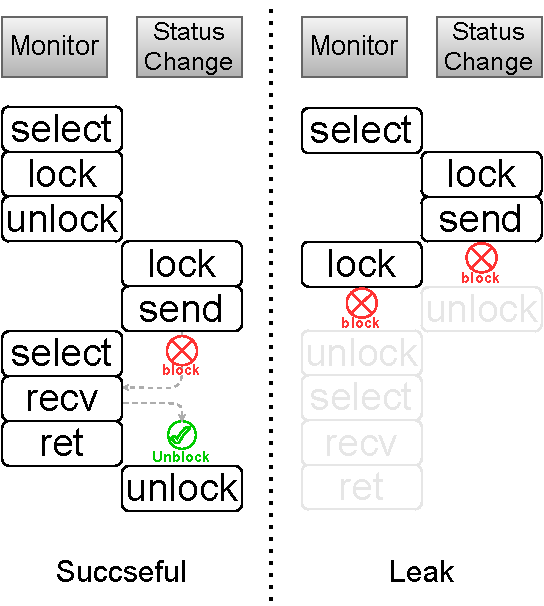
\includegraphics[width=.99\linewidth]{figs/execViz_moby.pdf}
\end{minipage}
\caption{Simplified version of bug \texttt{moby28462}}
\label{listing:moby28462}
\end{listing}


%\stcmtside{Explaining the example to motivate}
Listing \ref{listing:moby28462.minipage} shows a simplified version of a reported bug in Docker \cite{moby-28462-commit}.
%
An instance of the \texttt{Container} type (lines \ref{bugListing:containerType_start}-\ref{bugListing:containerType_end}) is created in the \texttt{main} function (lines \ref{bugListing:container_create_start}-\ref{bugListing:container_create_end}).
%
In line \ref{bugListing:main_go_monitor}, a goroutine is spawned to execute function \texttt{Monitor} that continuously checks the container status and returns once it receives from the container's channel (lines \ref{bugListing:Monitor_case_recv}-\ref{bugListing:Monitor_case_recv_ret}).
%
The default case of the \texttt{select} statement (line \ref{bugListing:Monitor_case_def}) allows \texttt{Monitor} to continue monitoring without getting blocked on the channel receive (line \ref{bugListing:Monitor_case_recv}).
%
Concurrent to the \texttt{main} and \texttt{Monitor} goroutines, another goroutine is created in line  \ref{bugListing:main_go_statChange} to execute function \texttt{StatusChange} which changes the status of the container by sending to the container's channel.
%
The container's lock is released after the send action completes and function returns (\texttt{defer} statement in line \ref{bugListing:statChange_defer_unlock}).
%


Native execution of this program terminates successfully without issuing any error or warning.
%
Based on the Go specification and memory model, there is no constraint on the goroutines spawned from the \texttt{main} function to join back before the \texttt{main} goroutine\footnote{In the remainder of the paper, we use \textit{main function} and \textit{main goroutine} interchangeably.} terminates.
%
A deadlock detector within the runtime periodically checks that the scheduler queues of all \textit{runnable} goroutines never become empty until the \texttt{main} goroutine terminates.
%
In other words, the runtime throws a deadlock exception when the \texttt{main} goroutine is blocked, and no other goroutine is in the queue to execute (\ie \textit{global deadlock}).
%
Since there is no blocking instruction in the \texttt{main} goroutine in listing \ref{listing:moby28462.minipage}, the program terminates successfully regardless of other goroutines' statuses.
%
However, this program suffers from a common bug in concurrent Go where one or more goroutines \textit{leak} (\ie, \textit{partial deadlock}) from the execution (\ie, never reach their end states).

%\stcmtside{Explain the deadlock (leak) situation that might get overlooked}
%Due to the non-determinism introduced by the runtime scheduler and application-level random features like \texttt{select}, many interleavings are feasible for concurrent execution of simple programs such as listing \ref{listing:moby28462.minipage}.
%
The right side of the listing displays a successful run and a leak situation of the program.
%
In the leak situation, first, the \texttt{Monitor} goroutine executes the \texttt{select} statement and, based on the available cases, picks the default case to execute.
%
Right before the execution of mutex lock (line \ref{bugListing:Monitor_case_def_lock}), the scheduler context-switches and the \texttt{StatusChange} goroutine starts its execution through which it holds the lock and blocks on sending to the channel (line \ref{bugListing:statChange_send}) since there is no receiver on that channel.
%
Upon blocking on send, the scheduler transfers back the control to the \texttt{Monitor} goroutine that tends to acquire the mutex, but because the mutex is already held by \texttt{StatusChange}, the \texttt{Monitor} goroutine also blocks.
%
The circular wait between the container mutex and channel prevents both spawned goroutines from reaching their end states and leaves the program in an unnoticed deadlock situation.
%
%\stcmtside{The thirst for novel and scalable debuggers}
%Widely used deadlock detectors such as Goodlock \cite{havelund-goodlock-spin00} are not applicable in Go since causes of Go deadlocks are resources (\eg, locking a locked mutex) or communication (\eg, sending on a full channel), or a combination of them (\eg, leaky interleaving of listing \ref{listing:moby28462.minipage}).
%
%In addition, due to the lightweight nature of goroutines, it is not uncommon to spawn thousands of goroutines in production software systems.
%
%Hence,  novel and scalable techniques are needed to enable realistic modeling of program behavior during execution.
%

\subsection{Concurrency Bugs in Go}
\label{sec:goBugs}
Based on a proposed bug taxonomy for Go \cite{tu-concurrentBugs-asplos19}, bugs are categorized separately based on their \textit{causes} (shared-memory vs. message-passing) and \textit{symptoms} (blocking vs. non-blocking).
%
Blocking bugs historically refer to situations where one or more processing units (\eg, goroutines) are blocked, waiting for an external signal to resume (\eg, leak situation in listing \ref{listing:moby28462.minipage}.
%
The observed causes of such blocking flaws in the context of Go are as follows:

\begin{itemize}
  \item \textit{Resource deadlocks}: Go inherits resource deadlocks from multithreaded languages like Java and C/Pthreads where goroutines are trapped in a circular wait for the resource (\eg, mutex) that is held by other goroutines.
  \item \textit{Communication deadlocks}: Synchronized (unbuffered) channels transmit values from one goroutine to another in a rendezvous fashion. The sender (or receiver) blocks until the receiver (or sender) is ready to receive (send). Misuse of channel operations might result in one or more goroutines waiting for a sender/receiver to unblock them forever.
  \item \textit{Mixed deadlocks}: The leak situation in listing \ref{listing:moby28462.minipage} is the example of such deadlocks where one goroutine is blocked on acquiring a resource that is held by another goroutine which is blocked on communication.
\end{itemize}

Similar to other concurrent languages, Go has non-blocking bugs such as data races and atomicity violations while introducing new bug idioms due to its new concepts such as anonymous functions \cite{tu-concurrentBugs-asplos19}.
%
This work focuses on blocking bugs (i.e., partial and global deadlocks).

%\stcmt{below: Application-level non-determinism makes debugging more difficult}
%\noindent{\bf Application-level non-determinism:\/}
In addition to the non-deterministic nature of concurrent languages caused by the scheduler and interaction between concurrent components, Go introduces some level of non-determinism at the application level.
%
The \textit{select-case} statement (similar to switch-case) allows the goroutine to wait on multiple channel operations.
%
The runtime picks one case pseudo-randomly among available cases (\ie, channel sends and receives that are ready to execute without blocking).
%
If none of the cases are ready, the executing goroutine is blocked unless there is a \textit{default} case.
%
The default case makes the select non-blocking and prevents the goroutine from waiting for unavailable communications.
%
Such random behavior expands the interleaving space, and it grows exponentially when nested selects are employed in conjunction with nested loops.
%
As a result, tracing the cause of a program's misbehaved execution becomes increasingly tricky.
%
Our observations (section \ref{sec:evaluation}) demonstrate that \textbf{select statements are in the core of rare bugs}.


\subsection{Accelerating Bug Exposure}
Blocking bugs are primarily caused by the non-deterministic decisions that the scheduler makes.
%
Such bugs may not manifest themselves in conventional testing and are difficult to reproduce.
%
Figure \ref{fig:rare_bugs} displays the histogram of 68 blocking bug kernels grouped by the number of trials that \goat takes to detect them.
%
Approximately 30\% of bugs required more than one execution to happen and be detected by \goat.
%
\textit{stress testing} is a common way to detect such rare bugs by exercising the scheduler and examine the program's behavior in many executions.
%
However, such testing is inefficient because some interleavings might get tested repeatedly while other feasible interleavings remain untested.
%
Researchers have proven that a small amount of randomness in each test execution can drastically reduce the number of iterations needed to find concurrency bugs \cite{emmi-delayBounded-popl11}.
%
For instance, random context-switches before synchronization/serialization operations in concurrent programs increases the probability of finding rare concurrent bugs \cite{burckhardt-depthBug-asplos10}.
%
In listing \ref{listing:moby28462.minipage}, a rare context-switch after the \texttt{select} statement in line \ref{bugListing:Monitor_select} causes the lock operation on mutex $m$ in line \ref{bugListing:Monitor_case_def_lock} of goroutine \texttt{Monitor} to \textit{block} goroutine \texttt{StatusChange} on locking $m$ in line \ref{bugListing:statChange_lock} and causing a deadlock.
%
Concurrency primitive usages (\eg, channel send/recv, mutex lock/unlock, select) are the \textit{critical points} in the program because their behavior directly impacts the blocking behavior of Go programs.
%
In \goat, we statically identify such critical points and inject \textit{yield} handlers before each concurrency primitive usage.
%
During execution, the handlers randomly decide if the current goroutine should yield to other goroutines to execute.
%
Results in section \ref{sec:evaluation} show that such simple yields are effective in detecting rare bugs.

\subsection{Testing Coverage Analysis}
\label{sec:coverage}
To demonstrate that testing has been thorough, \textit{coverage metrics} are defined to measure the progress of tests and specify testing termination conditions.
%
Coverage metric for the set of testing executions $\mathcal{T}$ is a set of \textit{requirements} $\mathcal{R}$ that should get covered during testing iterations.
%
We say requirement $R_i \in \mathcal{R}$ is covered during testing iteration $t_j \in \mathcal{T}$ if we can correlate an \textit{action} during execution of $t_j$ to $R_i$.
%
For example, in \textit{statement coverage}, which is a widely-used metric in testing sequential software, $R$ is the set of source locations (file and line numbers) in the target program.
%
$R_i$ is covered by test execution $t$ if the statement at location $R_i$ is executed in $t$.
%
The \textit{coverage percentage} of a test $\mathcal{T}$ is the ratio of the requirements covered by at least one execution over the number of all requirements ($|R|$).

Concurrent software testing frameworks perform testing iterations to explore the schedule space and expose flaws.
%
Depending on the class of target bug, different coverage metrics are proposed to quantify the quality of search space exploration.
%
\textit{Synchronization} coverage metrics such as \textit{blocking-blocked} \cite{edelstein2003contest}, \textit{blocked-pair-follows} \cite{trainin-followsCoverage-padtad09} and \textit{synchronization-pair} \cite{hong-syncTesting-issta12} defined requirements to cover during testing for exposing blocking bugs (\eg deadlocks).
%
%\textit{Memory access} coverage metrics such as PSet \cite{yu-pser-isca09} and def-use \cite{yang-defuse-issta98} focuses on data-access related bugs such as atomicity violation or data races.
%
For example, the synchronization coverage model in \cite{edelstein2003contest} defines \textit{blocking} and \textit{blocked} requirements per each synchronized block (\ie mutually exclusive section of the code that is protected by a lock).
%
The purpose of this requirement is to check if a test can report when there is a lock contention for two or more threads entering the synchronized block.
%
That is, a thread is either \textit{blocked} from entering the synchronization block or \textit{blocking} other threads from entering by holding the lock.
%



\begin{figure}[]
\centering
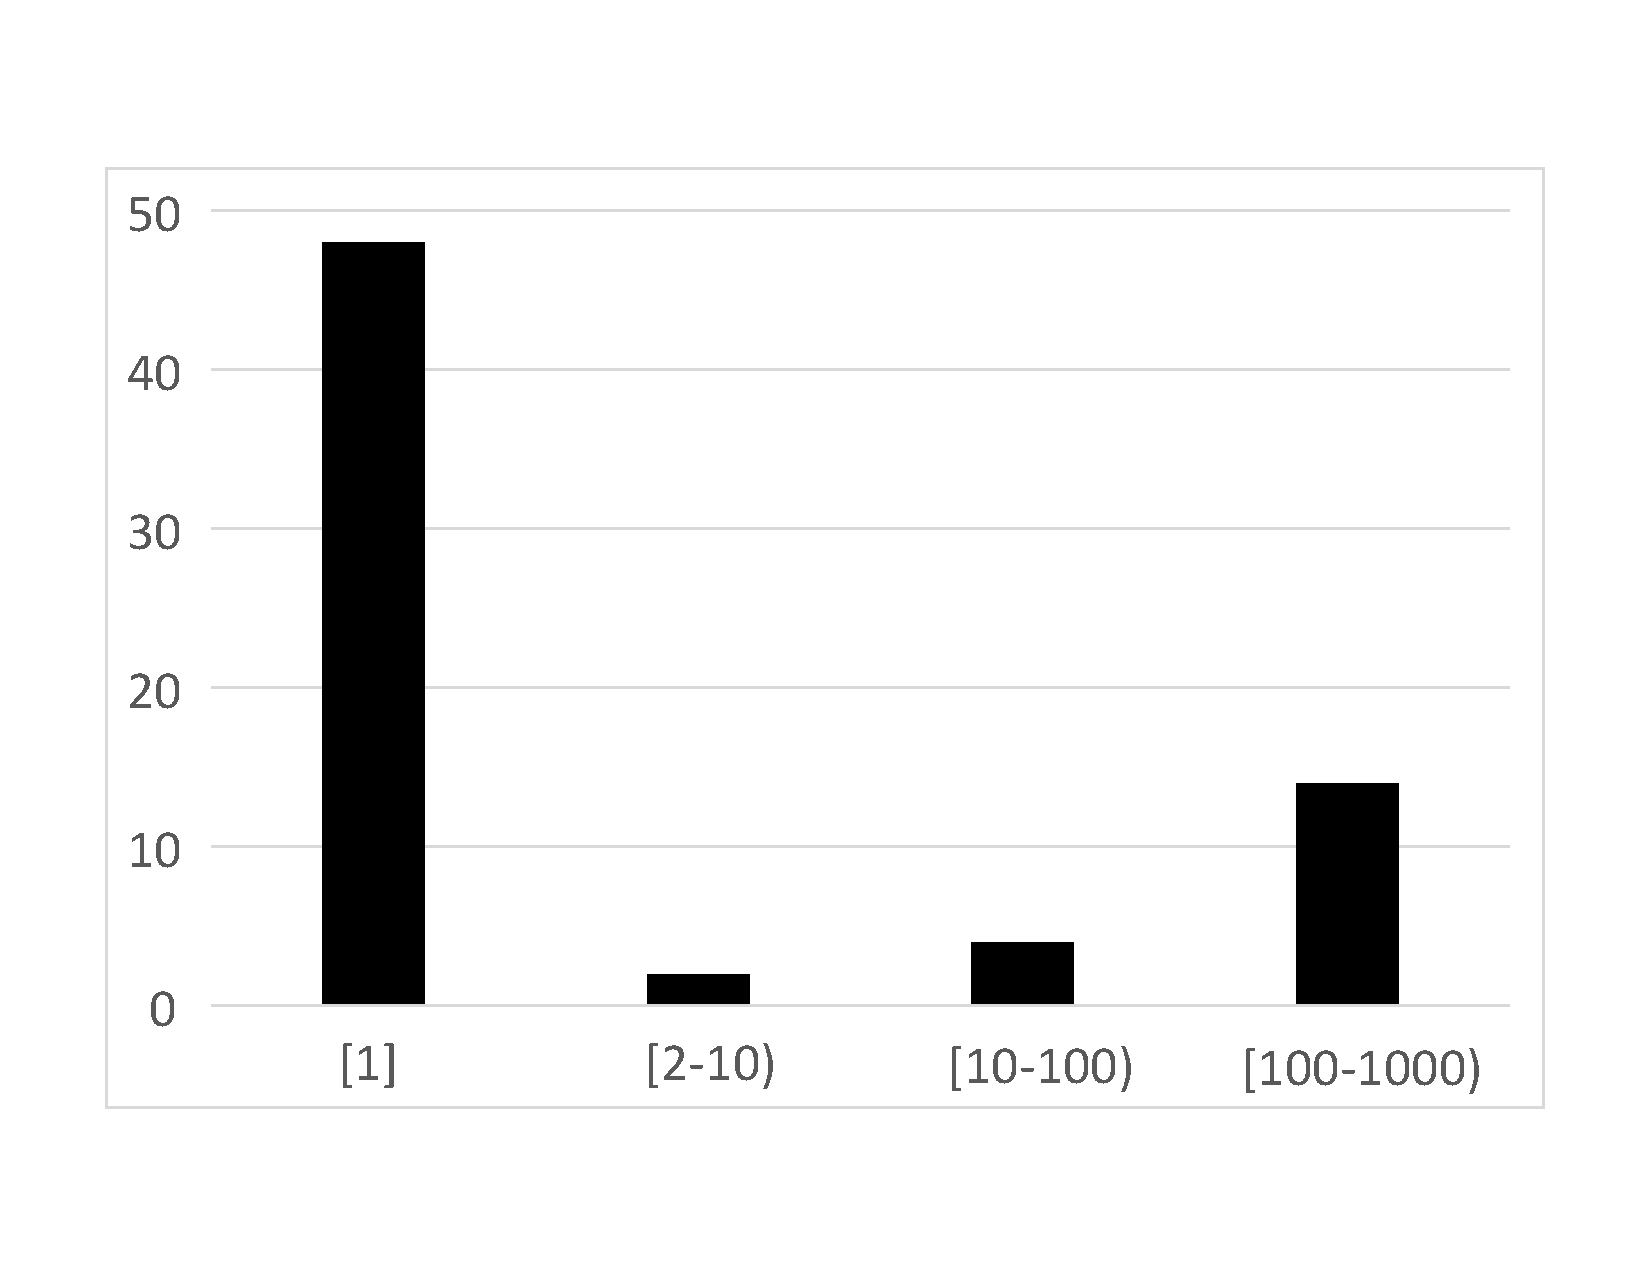
\includegraphics[width=0.8\linewidth]{figs/coverage_motivation.pdf}
%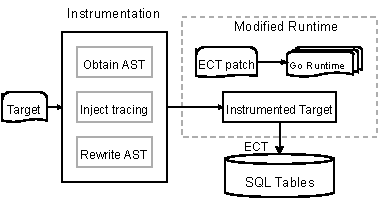
\includegraphics[]{figs/overview.png}
%\includegraphics[]{figs/overv}
\caption{Distribution of number of trials for \goat (D0) to detect 68 blocking bugs in GoKer~\cite{yuan-gobench-cgo21}}
\label{fig:rare_bugs}
\end{figure}


The existing concurrency coverage metrics are primarily in the context of Java and C/Pthreads.
%
They are not directly applicable to languages like Go as such languages have different concurrency primitives and semantics.
%
Novel coverage metrics are required to enable the quantification of interleaving space exploration.
%
Bron et al.,\cite{bron-appSyncCov-ppopp05} enumerates four major characteristics for coverage metrics to gain acceptance:
\begin{enumerate}
  \item \textbf{Static model:} A static model of requirements from the given program should be constructed by instrumenting the source code. The model should be well-understood by the developer or tester before execution. The model should maintain covered requirements during testing executions.
  \item \textbf{Coverable and measurable requirements:} The absolute majority of requirements should be realistic enough to be \textit{coverable} during testing. For a few that are not coverable (due to program semantics) or not \textit{measurable} (because of technical limitations), the developer should be aware of the reason.
  \item \textbf{Actions for uncovered requirements:} After testing terminates, every uncovered requirement should yield an action (\eg, extending testing iterations or removing dead code from the program, thus removing uncoverable requirements)
  \item \textbf{Coverage satisfaction:} Some action should be taken upon reaching a threshold of coverage percentage (e.g., testing phase termination when reaching 100\% statement coverage)
\end{enumerate}

Defining a new coverage metric to satisfy the above characteristics requires an accurate and proper mental model of target bugs.
%
Using the \goat's infrastructure, we deep studied the underlying causes of many bugs, including GoKer benchmark~\cite{yuan-gobench-cgo21} and proposed a set of coverage requirements that enables extensive analysis of dynamic behavior of concurrency primitives under various scheduling scenarios.
%
In section \ref{sec:covreq}, we describe our proposed coverage metric for testing concurrent Go, which are extensible to all concurrent languages.


\section{GOAT: Debugging}
\label{sec:design}
\stcmtside{1 paragraph about general design}
\stcmt{
- ECT Collection
\\
-Instrumentation
\\
- Deadlock Detection
\\
- Injecting Delays at critical points

}
\begin{figure}
\centering
  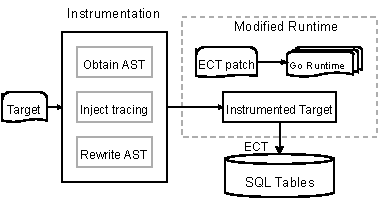
\includegraphics[width=.95\linewidth]{figs/overview.pdf}
  \caption{Framework Overview}
  \label{fig:overview}
\end{figure}


\subsection{Execution Concurrency Tracing (ECT)}
\label{sec:ect}
When enabled, the execution tracer package captures and compresses an execution trace (ET).
%
Upon program termination, the ET is flushed to an IO buffer.
%
The decompressed ET is a sequence of events with a precise nanosecond-precision timestamp and a stacktrace for most events (total of 49 events \cite{goParserSource}, categorized and summarized in table \ref{tab:events}).
%
Through a one-time patch, we extend and enrich ETs with \textit{concurrency usage} events to obtain \textit{execution concurrency traces} (ECT):
\begin{itemize}
    \item \textbf{Channel:} For each channel operation (make, send, receive, close), ECT includes an event with the full stack trace of up to application source line number, a unique id to distinguish between different invocations (e.g., in a loop), and an argument to show the type of operation (blocking/non-blocking based on the state of channel buffer). Upon creation, a unique id is assigned to each channel to keep track of its operations during execution.
    \item \textbf{Mutex, WaitGroup \& Conditional Variables:} Similar to channels, we assign a unique id to each concurrency object and emit an event for each of their operations (lock, unlock, add, wait, signal, broadcast). We also distinguish between non-blocking operations (e.g., free mutex) and blocking ones.
    \item \textbf{Select \& Schedule:} The scheduler and the \textit{select} structure introduce non-determinism to the execution. We keep track of the decisions made by the scheduler and select statements to obtain an accurate \textit{decision path} during execution.
\end{itemize}

Having a precise model of concurrency primitives such as the ECT enables interesting analysis in offline space.
%
Valuable knowledge such as frequency of concurrency usage per goroutine, blocking/non-blocking execution of concurrency primitives, and the last event executed by each goroutine (for leak detection) can get extracted from ECT.


\begin{table}[b]
    \centering
        \begin{tabular}{|l|l|}
        \hline
        \rowcolor[HTML]{C0C0C0}
        \multicolumn{1}{|c|}{\cellcolor[HTML]{C0C0C0}\textbf{Category}} & \multicolumn{1}{c|}{\cellcolor[HTML]{C0C0C0}\textbf{Description}} \\ \hline
        Process & Indication of process/thread start and stop \\ \hline
        GC/Mem & Garbage collection and memory operation events\\ \hline
        Goroutine & Goroutines events: create, block, start, stop, end, etc. \\ \hline
        Syscall & Interactions with system calls \\ \hline
        Users & User annotated regions and tasks (for bounded tracing) \\ \hline
        Misc & System related events like futile wakeup or timers \\ \hline
        \end{tabular}

    \caption{Event categories by the Go execution tracer}
    \label{tab:events}
\end{table}



\subsection{Critical Points}
\label{sec:critical}

Through statically traversing the AST of any target package (e.g., files of the “main” package), goat gathers a set of line numbers where concurrency functions are used. These points (aka critical points) are the points where a context switch might drastically change the concurrency behavior of the program and trigger an undiscovered bug. Here are the AST nodes that represent a critical point:
Go: ast.Node GoStmt   (example: go func() // spawning a new goroutine)
Send: ast.Node SendStmt     (example: channel <- x)
Recv: ast.Node UniExprStmt(op=”<-”) (example:  <- channel)
Mutex, WaitGroup, CondVars: ast.Node CallExpr (example: xxx.Lock())
Xxx.Lock()
Xxx.Unlock()
Xxx.Add()
Xxx.Wait()
Xxx.Signal()
Xxx.Broadcast()
Careful adjustment is required for Select and Range statements that have send/recv as their children in the AST.

\subsection{Instrumentation}
\label{sec:instrument}
Identifying “critical points”:
Instrumentation: goat inject goat\_handler() calls before the critical point nodes. Goat\_handler() can be a call to any desired scheduler-manipulator. For instance, currently it calls an external function that randomly and boundedly yield to all other runnable goroutines (i.e., call gosched()). It gives us the flexibility to experiment different kinds of random and systematic (e.g., coverage-guided) scheduler-manipulation from an external function and environment variables without touching goat or goatlib API. In addition to critical points, goat adds four more line to the beginning of main function:
Import goat
goat\_done := goat.Start() // Start() initializes goat and starts tracing. It also creates and returns a channel for signaling the Stop()
go goat.Watch(goat\_done) // spawns a new goroutine as a watcher for liveness of the program (in case of global deadlocks or infinite loop). Watch() either receives from done and performs : goat\_done <- true, or timeouts and stop tracing, and terminates.
defer goat.Stop(goat\_done) // after the main ends, Stop() is called to send a value to the watcher goroutine and signaling that the program is finished. Then it waits to receive the ack from watcher, then stops tracing and terminates.
Trace collection: Currently, goat can collect a plain ECT from the native execution and also ECTs from executions with manipulated scheduler.
Deadlock detector: After the program terminates, goat queries the database to distinguish main goroutines and application spawned goroutines from background goroutines (runtime, tracing, etc.). Then it checks if all application goroutines ended with “GoEnd” (otherwise there is leak – partial deadlock) and if the main goroutine is ended with “GoSched” (otherwise there is a global deadlock since main did not finish).


\subsection{Deadlock Detection}
\label{sec:deadlock}

\begin{itemize}
  \item \textbf{Identifying Root, Main and App goroutines:}
  In the lifetime of a program, the runtime system creates new goroutines or pick from the pool of dead goroutines to perform various tasks such as bootstrapping the program, garbage marking and sweeping, and tracing.
  %
  \goat also adds extra goroutine to \textit{watch} the main goroutine in case of blockage of the main goroutine.
  %
  These extra goroutines are captured in the tracing but we are not interested in studying them as our main focus is the main application (or test) and all application-level goroutines.
  %
  By checking the stack of creation location, \goat prune the goroutine tree from unimportant goroutines.
  %
  We only keep and analyze events from the execution of main goroutine and all G such that ancestor(G) = main.
  \item \textbf{Final Event:}
  ECT captures end-to-end sequence of events for each goroutine representing its lifetime behavior.
  %
  If tracing is enabled, every application goroutine invokes the tracer to capture $GoEnd$ before finishing its execution and exit (change status from \textit{grunnable} to \textit{gdead})\cite{goexit-line-of-code}.
  %
  Before the main function returns (\ie exits), it calls the scheduler (through runtime.Gosched() invocation which captures $GoSched$ event) to hand over the control to the root goroutine to finish up program execution.
  %
  Since we instrument the application to stop tracing when main returns (through calling trace.Stop()), $GoSched$ would be the last event captured for the main goroutine if it returns succesfully.
  %
  We call an execution \textbf{successful}, if below conditions hold
  \begin{itemize}
    \item (1) all goroutines spawned in the main goroutine has $GoEnd$ as their final event
    \item (2) the final event of the main goroutine is $GoSched$ with \texttt{runtime.traceStop} on top of its stack.
  \end{itemize}
  If either of above conditions does not satisfy after program execution, a \textbf{deadlock} happens because it shows that there are one or more goroutine that did not reach its final state.
  %
  A one-line query to the application database retrieves the final event of each executed goroutine.
  %

\end{itemize}



\section{GOAT: Coverage}
\label{sec:coverage}
\stcmt{intro to coverage}
\begin{itemize}
  \item A coverage metric specify a set of requirements on a target program which a complete test should satisfy
  \item A test requirement is a condition over a target
  program
  \item An execution covers a test requirement when the execution satisfies the
  test requirement
  \item The coverage level of a test (i.e., a set of executions) is the ratio of the test requirements covered by at least one execution to the number of all test requirements
  \item A coverage metric is used for assessing progress of a test and measure the quality of a test (to assess whether a test is sufficient or not)
\end{itemize}


–
–
–




\begin{figure}
\centering
  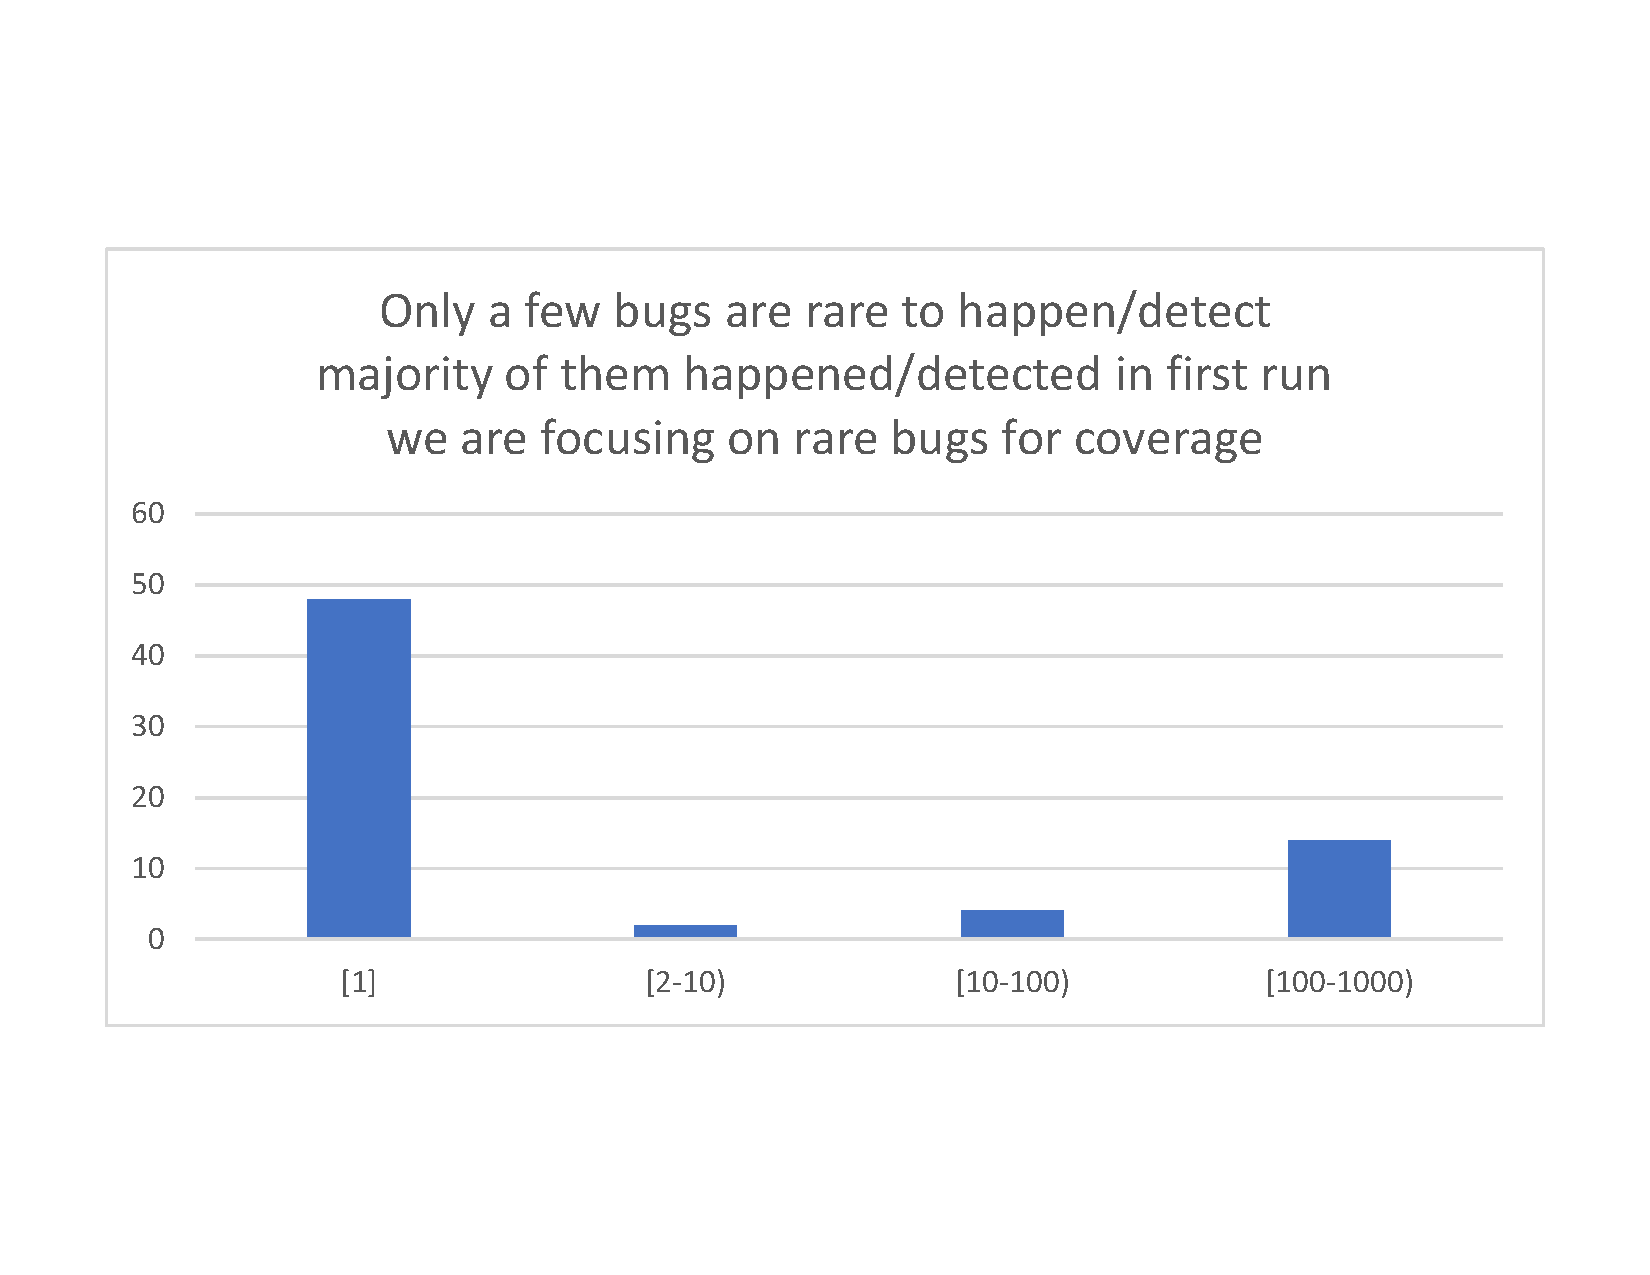
\includegraphics[width=.95\linewidth]{figs/coverage_motivation_tentative.pdf}
  \caption{focusing on rare bugs}
  \label{fig:rare_bugs}
\end{figure}

\begin{itemize}
  \item Limitations of current concurrency coverage criterias
  \item what it takes to define a good coverage metric
  \begin{itemize}
    \item thorough observation of target bugs, their symptoms, their causes and fixes.
  \end{itemize}
  \item
\end{itemize}

\subsection{Coverage Idea}

Figure \ref{fig:rare_bugs} shows that even a drastically simplified versions

we define a coverage metric to quantify the quality of tests

we inject random delays which is effective in testing different scenarios

we measure the coverage for our testing using the tracing mechanism



we

Existing concurrent coverage metrics target either synchronization primitives or memory access for Java. In Java, locks and other serialization techniques like conditional variables and semaphores usually provide mutual exclusion and memory protection (i.e., no “direct” communication between threads are involved. In Go, a goroutine can directly unblock another goroutine)
\\
-	For example in Java,  thread A either is blocked from entering a critical section (or mutually exclusive section) protected by lock L or is blocking other threads (e.g., thread B) from entering the critical section.
\\
If, during testing (e.g., exploring schedule-space and interleavings), one thread never gets blocked and always blocks other goroutines on a lock operation, it is often the case that there is a possible untested and important interleaving. Blocked/blocking coverage model is the basis of existing synchronization coverages. A 100\% coverage on operation e is achieived when each thread t\_i performs e in blocked and blocking way, at least one each.
-	Test coverage analysis: defining a set of tasks and check that each task is covered in testing phase. A coverage metric is defined based on the tasks to measure quality and completeness of testing.
-	Superior coverage metrics like source-line coverage and branch coverage are popular because they have four major characteristics:
\begin{itemize}
  \item The metric should be well-understood by the developer or tester. Models to run tasks for measuring metrics should construct statically by instrumenting the source-code.
  \item All tasks should be coverable. For a few that are not (due to technical limitations or program semantics), a review process is required.
  \item Every uncovered task should yield an action: add more tests or remove dead code (re-design)
  \item Some action should be taken upon reaching a threshold of coverage(e.g., testing phase termination when reaching 100\% statement coverage)
\end{itemize}

-	In addition to blocked/blocking, other synchronization coverage metrics like sync-pair, follows, PSet, HaPSet are defined to measure quality of interleaving-space testing of concurrent software, mostly in Java and C++.
\\
-	Another important factor is the importance of common bug scenarios based on the platform specification and target class of bugs. Coverage metrics that are defined for races or atomicity-violation in Java are not applicable for blocking bugs (non-memory-access bugs) in Go. Hence, new coverage metrics are required.

\subsection{New coverage models}
Based on my observations from studying GoKer bugs using the GOAT infrastructure, here is my proposal for a set of coverage models to measure the quality of interleaving-space search of GOAT random and bounded schedule permutation:
\begin{itemize}
  \item The Select-case statement is the major cause of rare bugs specific to Go. Multiple blocking actions (send/recv) might get blocked on a select statement. Once one or more becomes available, Go picks one “randomly”. A default case make select “unblocking”. When no blocking case is available, the default case let the goroutine to make progress. GOAT and ECT are capable of identifying the select statement behavior (e.g., which case have been selected in each execution of select).
  \item Unlike lock operations that might be blocked  or blocking, channel sends and receives are blocked or “unblocking”. Channel sends (receives) blocks a goroutine if the receiver (sender) is not ready or unblocks a goroutine if the receiver (sender) is already waiting. A channel send/recv might also be of type no-op (for buffered channels).

\end{itemize}

-	While existing synchronization coverages often ignore unlocks, I think unlocks are also important because they might (or might not) “unblock” a waiting goroutine (unblocking/no-op)
\stcmt{Why I think this is good?}
- It exploits the enhancement I made for Go tracer.
- The proposed coverage model idea is strong because:
- It follows the four rule of popular coverage metrics
- It is based on a thorough study of GoKer bugs
- I can generate a interesting tables to show the impact of the random scheduler-perturbations.
- It is novel and adds some scientific aspect to my thesis.

\subsection{Implementation}
It is crucial to maintain a static model of goroutines and coverage metrics during testing executions. I obtain such model in two ways:
-	Statically: The concurrency usage (ie, source line numbers that perform actions go/send/recv/lock/unlock/wait/done/sig/bcast/select) is obtained from traversing the source AST. Such concurrency usage model has two purposes:
- Critical points to inject sched\_yield before them.
- A pre-execution model of testing tasks. During testing phase, we map each source line with its corresponding action to an event in ECT based on its call-stack.
-	Dynamically: A good test run is required to obtain some models dynamically. (I will explain GGTree and stack later. Why do we need GGTree?)




\begin{figure}
\centering
  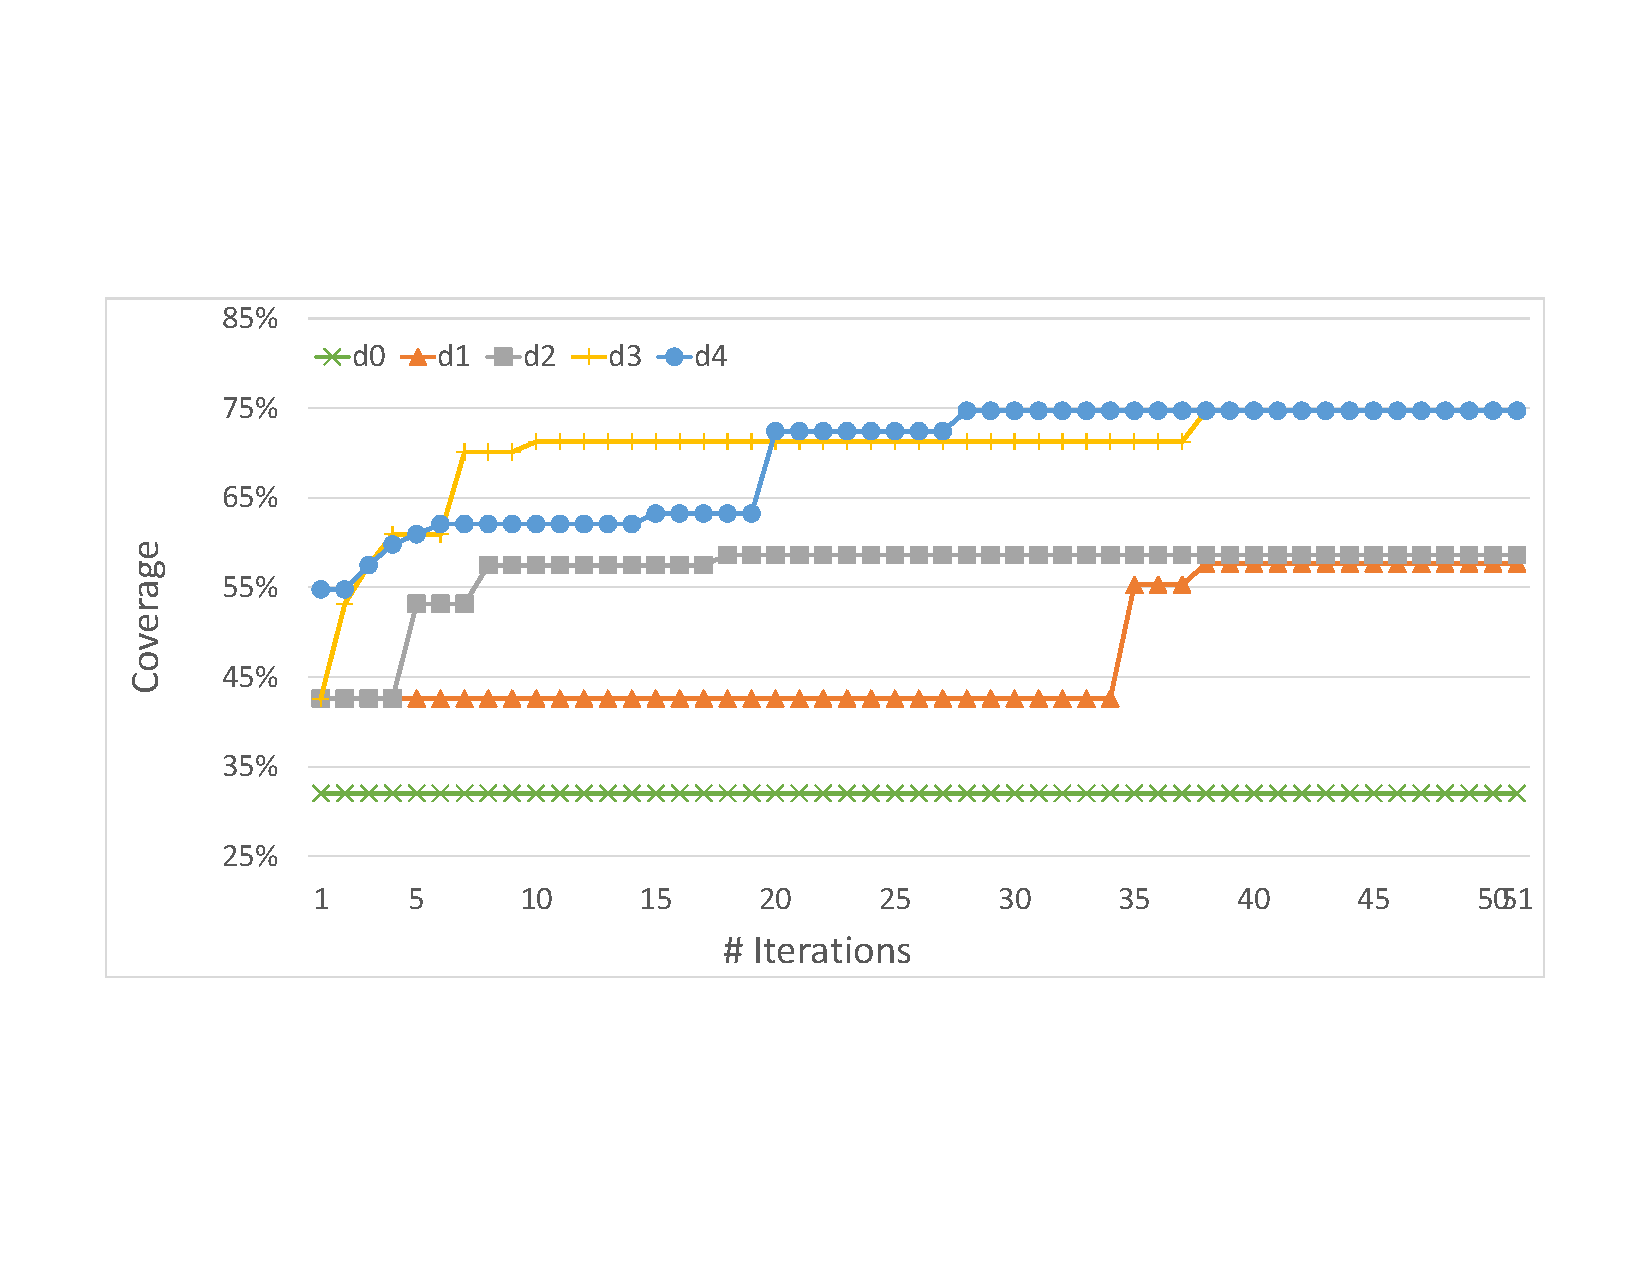
\includegraphics[width=.95\linewidth]{figs/coverage_etcd7443.pdf}
  \caption{etcd7442 coverage}
  \label{fig:etcd_coverage}
\end{figure}


\begin{figure}
\centering
  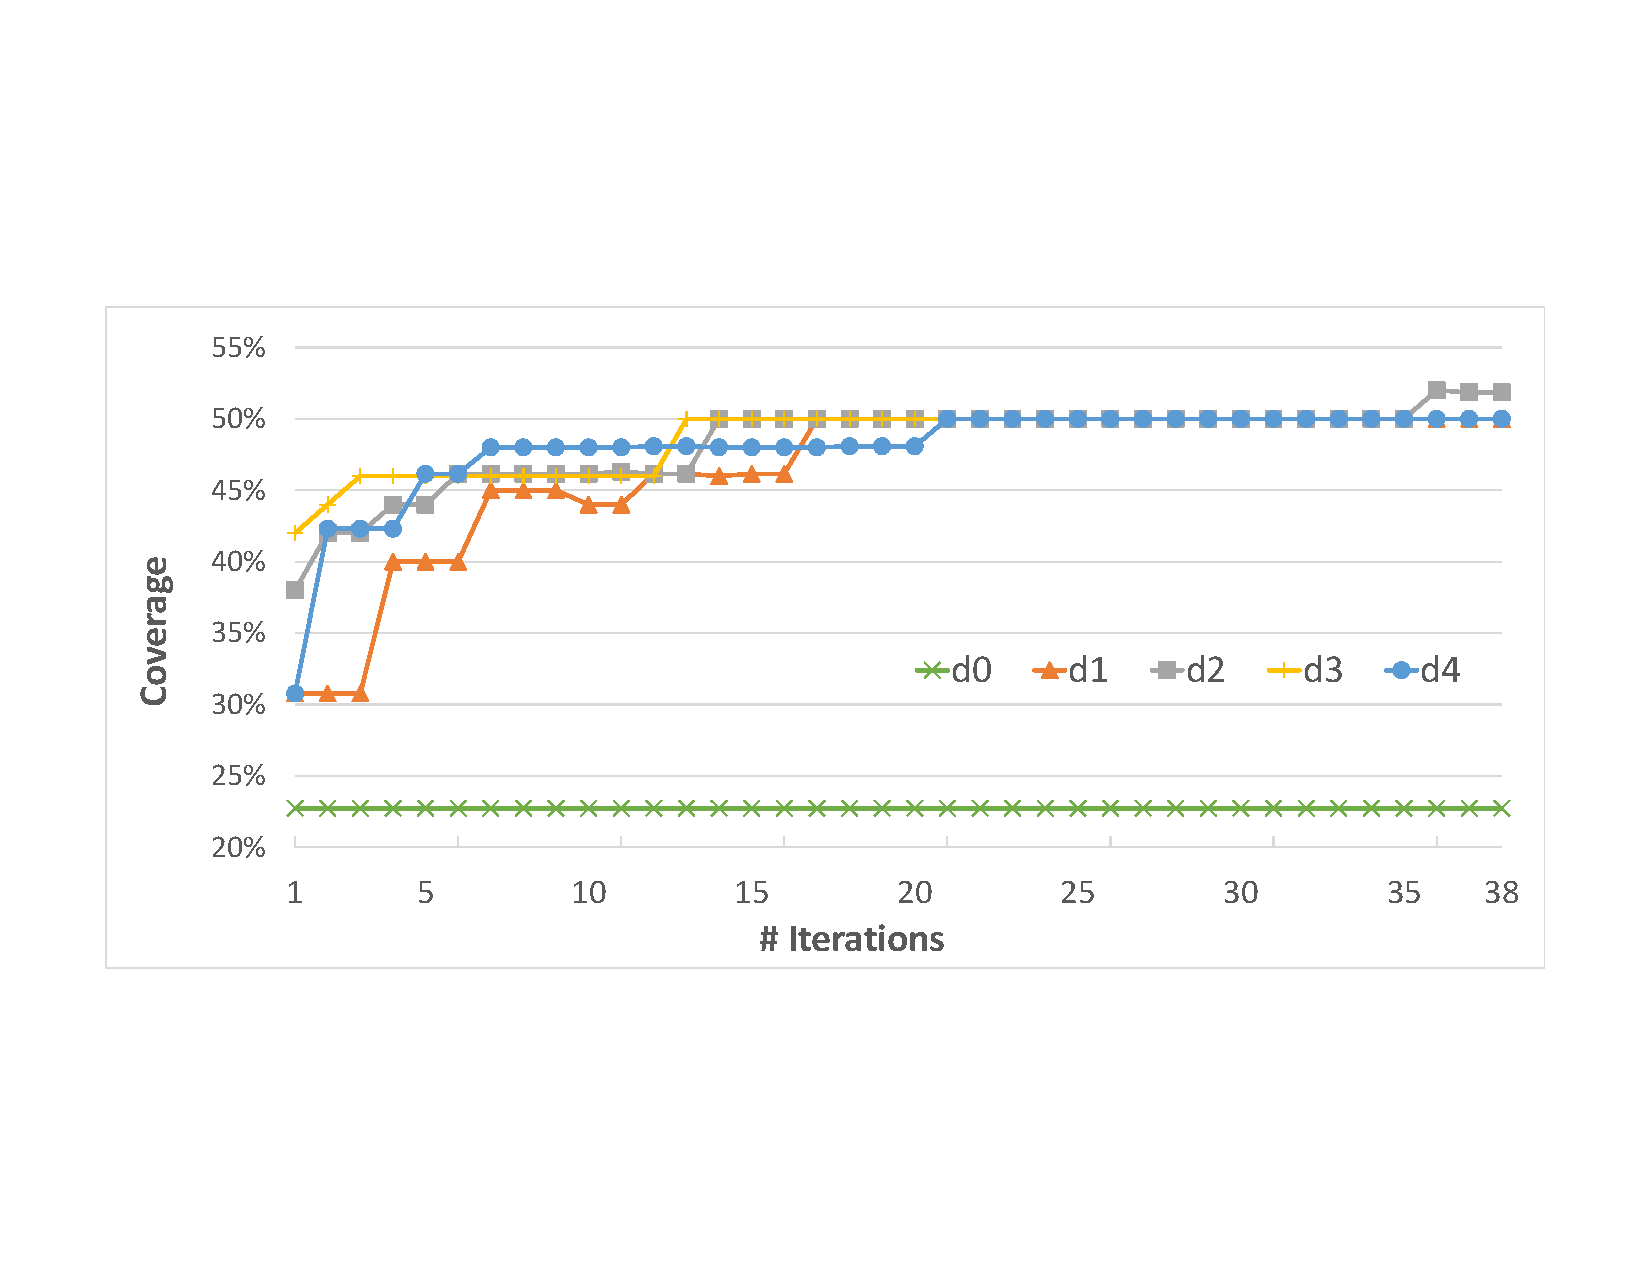
\includegraphics[width=.95\linewidth]{figs/coverage_kubernetes11298.pdf}
  \caption{kuberenetes11298 coverage}
  \label{fig:kubernetes_coverage}
\end{figure}











\subsection{Coverage Definition}
test coverage analysis
how well we are testing the program
systematic testing
how well we are testing
what is the minimum coverage requirement for exposing the bug

why are we defining a new coverage metric?
because we want to quantify the quality of concurrent software testing for a language like go

to do


\section{Related Work}
\label{sec:related}
For correctness of CSP-based concurrent languages like Go, Ng and Yoshida \cite{ng-dl-cc16} proposed a static tool to detect global deadlock in Go programs using choreography synthesis.
%
Later, Stadtmuller et al. \cite{stadtmuller-minigo-aplas16} proposed a static trace-based global detection approach based on forkable regular expressions.
%
Lange et al. proposed more static verification frameworks for checking channel safety, and liveness \cite{lange-fence-popl17}, and behavioral model checking \cite{lange-staticType-icse18}.
%
Both methods approximate Go programs with session types and behavioral contracts extracted from their SSA intermediate representation.
%
The mentioned work has limitations for handling dynamic (e.g., in-loop) goroutine or channel creation, and programs with many goroutines. Besides, the rate of generated false positives is high.
%
As dynamic (runtime-level) analysis approaches, Zhao et al. \cite{zhao-occam97} introduced a heuristic-based runtime monitoring approach for deadlock detection in Occam programs.
%
Sulzmann and Stadtmuller proposed a dynamic verification approach for synchronous (unbuffered) channels \cite{sulzmann-corr17}, and a vector-clock-based approach for asynchronous channels \cite{sulzmann-twophase-2018}.
%
Although they may support a larger subset of the Go language, they only focus on channels as the root cause of deadlocks and evaluated on relatively small examples.
%
Also, they usually do not scale for applications with thousands of goroutines and LOC \cite{dilley-empirical-saner19}.

%
Researchers have applied different systematic testing methods \cite{thomson-concurrencyTesting-ppopp14} to reduce the interleaving space to explore effectively and efficiently.
%
Delay-bounded \cite{emmi-delayBounded-popl11,burckhardt-depthBug-asplos10} and preemption-bounded \cite{madanlal-preemptionBound-pldi07} techniques systematically ``fuzz'' the scheduler to equally and fairly cover feasible interleaving.
%
Other tools like Maple \cite{yu-maple-oopsla12}, CalFuzzer \cite{joshi-calfuzzer},  and ConTest \cite{edelstein2003contest} \textit{actively} control the scheduler to maximise a pre-defined concurrency coverage criterion \cite{hong-syncTesting-issta12} or the probability of bug exposure \cite{burckhardt-depthBug-asplos10}.





\bibliographystyle{IEEEtran}
\bibliography{bibs}


\end{document}
